\section{Evaluation}
\label{sec:evaluation}

This chapter sets out the evaluation design for Intent-Conditioned Value Projection as a decision model for the Internet of Value, and reports the preliminary numbers from the current benchmark run. The empirical question is the one posed in RQ3 of Chapter \ref{sec:aims}. To what extent does ICVP improve decision quality, evidence relevance, and auditability across NFT, productive-asset, and treasury-governance scenarios, compared with single-dimensional and fixed-weight valuation baselines? The chapter is organised around framework validation, not around a comparison between commercial language models. Model choice is held fixed across configurations within each task and is treated as a configuration variable, not as the object of study. The figures in the tables that follow are preliminary. They come from partial runs with the reference panel and from a snapshot of the evidence space, and they will be revised once the full benchmark is rerun with finalised model versions and final evidence snapshots. A specific figure that is a placeholder rather than a measurement is marked as such.

\subsection{Evaluation design}

The evaluation is a controlled framework-validation benchmark. Its purpose is not to prove that ICVP is universally optimal, that value has an objective ground truth, or that a language model is correct. It tests the narrower claim that the mechanisms proposed in this thesis improve decision support on tasks where intent changes what evidence matters and what the valuation dimensions mean. The benchmark supports ICVP if the full configuration outperforms reduced alternatives that remove its load-bearing mechanisms.

The evaluation uses twelve tasks distributed across three domains. Four tasks address a Pudgy Penguin NFT held under different intents, four tasks address stETH as a productive asset, and four tasks address Polkadot OpenGov treasury proposals under public-resource stewardship. Each task fixes an asset or proposal, a stated intent, and the action under consideration. The set is small enough to evaluate carefully and broad enough to expose whether ICVP generalises beyond a single asset class. The fixed task set also makes the comparison controlled: the asset, intent, action, evidence snapshot, model family, prompt budget, and scoring rules are held constant within each task while the valuation configuration is varied.

The evaluation compares three configurations. The full ICVP configuration retrieves evidence under the intent-specific projection $P_i$, instantiates Availability, Durability, and Utility under the intent-specific instantiation $\Phi_i$, applies the operational aggregation $g_i$, and emits a valuation trace with deterministic validation. The single-dimensional baseline collapses each task to its dominant visible signal. For NFTs this is floor price, listing depth, rarity rank, recent sales, or access signal depending on the task. For stETH it is peg, liquidity, yield, or protocol risk depending on the task. For treasury proposals it is requested amount, visible community sentiment, team reputation, or perceived utility depending on the task. The fixed-weight baseline keeps the Availability, Durability, and Utility decomposition but removes intent-conditioned projection and dimension instantiation. It uses one fixed weight vector across all tasks and domains and pulls evidence from a generic asset profile rather than from an intent-specific projection. This isolates the contribution of the projection $P_i$ and the instantiation $\Phi_i$ from the contribution of the three-dimensional decomposition.

\subsection{Validation logic}

The benchmark treats the baselines as reduced comparison models rather than as competing complete systems. The single-dimensional baseline removes the A/D/U decomposition, intent-conditioned evidence projection, trace validation, and the explicit \textit{defer} behaviour for incomplete evidence. The fixed-weight baseline keeps the A/D/U taxonomy but removes intent-conditioned projection and intent-specific dimension instantiation. A positive result for ICVP therefore has a specific interpretation: it suggests that decision support improves when the system first projects evidence by intent, then instantiates A/D/U under that intent, records provenance in a structured trace, and refuses confident \textit{proceed} recommendations when required evidence is missing, stale, conflicting, or untraceable.

The quantitative claims are tied to this validation logic. ICVP is supported on this benchmark if, relative to both reduced baselines, it improves decision agreement and macro-F1 against the expert reference labels, reduces the false-proceed rate, improves evidence relevance precision and recall against expert-marked evidence, improves A/D/U mapping quality against expert median scores and dimension-content ratings, improves trace and provenance completeness, and remains more robust under missing, conflicting, or injected evidence. These claims do not establish universal optimality. They establish that the mechanisms defended by the thesis are useful on a controlled set of heterogeneous Internet of Value tasks where reduced valuation models are expected to fail.

\subsection{Expert reference protocol}

Three independent evaluators with relevant blockchain expertise act as a reference panel. Eligible evaluators must have practical or research experience with at least one of NFT markets, DeFi liquid staking, DAO or OpenGov treasury evaluation, blockchain analytics, or smart-contract risk assessment. Before annotation, evaluators are screened for conflicts of interest. They must disclose direct holdings, employment, advisory relationships, funded work, governance participation, or personal involvement connected to the specific asset, protocol, collection, proposal, or proposer being evaluated. A disclosed material conflict excludes the evaluator from that task or requires replacement before the final benchmark run.

Evaluators receive the task description, the stated intent, the action under consideration, and the frozen evidence snapshot. They do not receive ICVP or baseline outputs during annotation. The annotation form asks for a decision label in $\{\textit{proceed}, \textit{defer}, \textit{decline}\}$, A/D/U scores under the stated intent, confidence, evidence items considered necessary, evidence items considered irrelevant or distracting, missing evidence, conflicts in the evidence, hard constraints, and a short rationale. In a second scoring pass, after the independent reference labels are fixed, evaluators rate whether each configuration's proposed A/D/U mapping correctly expresses the intent-specific meaning of Availability, Durability, and Utility for the task. Configuration identifiers are masked during this mapping-quality pass where the trace format permits masking.

The reference decision for a task is the majority label across the three evaluators. The reference A/D/U scores are the median scores. Evidence relevance is scored against the union of evidence items marked important by at least two evaluators, with single-evaluator evidence flags retained for sensitivity analysis. Disagreement is treated as uncertainty rather than as annotation failure. Label disagreement, A/D/U score spread, and rationale divergence are reported alongside performance, and high-disagreement tasks are expected to favour lower confidence or \textit{defer} rather than forced certainty. We treat expert assessment as a reference judgement rather than as absolute ground truth, and we use the term \emph{reference} rather than \emph{ground truth} throughout this chapter.

\subsection{Metrics}

The metrics are organised around three concerns. Decision quality is measured by agreement with the reference decision, by macro-F1 over $\{\textit{proceed}, \textit{defer}, \textit{decline}\}$, by false-proceed rate, and by deviation of A/D/U component scores from the expert median. Evidence relevance is measured as precision, recall, and distractor inclusion. Precision is the fraction of trace evidence items that match expert-marked relevant evidence. Recall is the fraction of expert-marked relevant evidence represented in the trace. Distractor inclusion is the fraction of expert-marked irrelevant evidence included in the trace. A/D/U mapping quality is scored separately by asking whether the dimension contents match the asset class, stated intent, and action context. Auditability is measured by trace completeness, provenance completeness, presence of confidence and hard constraints, and by the rate at which the deterministic validator accepts the trace. Computational overhead is reported separately as latency and cost per task. The false-proceed rate matters most because in the Internet of Value a wrong \textit{proceed} can be more harmful than a conservative \textit{defer}.

\subsection{Statistical analysis}

The benchmark size is intentionally small and expert-intensive, so the statistical analysis is descriptive and paired rather than framed as a broad population estimate. For proportions such as decision agreement, false-proceed rate, validator acceptance, provenance completeness, and robustness pass rates, the final report will include exact binomial confidence intervals. Where the same tasks are scored under two configurations, paired label outcomes will be compared with McNemar's test or an exact paired test when the discordant count is too small for the asymptotic approximation. Macro-F1 will be reported with paired bootstrap confidence intervals over tasks. Continuous or ordinal scores, including A/D/U component error, evidence relevance, trace completeness, and A/D/U mapping quality, will be reported with bootstrap confidence intervals and paired task-level differences.

Inter-rater agreement is reported to show how stable the reference panel is. Decision labels are summarised with Fleiss' $\kappa$. Ordinal A/D/U scores and ordinal mapping-quality ratings are summarised with Krippendorff's $\alpha$ or an equivalent ordinal agreement statistic. These agreement measures do not turn expert judgement into objective truth. They indicate whether the benchmark tasks are consensus-friendly or intrinsically contested. With $n=12$, the evaluation is underpowered for broad population-level claims, and statistically non-significant paired differences will not be interpreted as evidence of no effect. The evidential standard is convergence across paired direction, effect size, confidence intervals, and mechanism-specific failure analysis.

\subsection{Reproducibility and artifacts}

The final benchmark run will freeze all evidence snapshots before model execution. Each evidence item will be stored with source URL or API endpoint, retrieval timestamp, content hash, source type, freshness limit, and provenance flags. Each run will record the model identifier, model version or deployment date where available, prompt template version, tool adapter version, retrieval configuration, required-evidence schema version, validator version, scoring-script commit hash, and random seed or sampling settings. The primary output artifact for each configuration and task is the trace JSON, including selected evidence, excluded evidence, instantiated A/D/U fields, decision, confidence, hard constraints, validation result, and provenance.

The dissertation artifact package will include the task definitions, evaluator instructions, blank and completed annotation forms where publication is permitted, frozen evidence manifests, required-evidence schemas, trace JSON files, validation logs, and scoring scripts. If source licenses or privacy constraints prevent releasing the full evidence text, the release will include hashes, timestamps, URLs, and extraction instructions sufficient to reproduce the snapshot as closely as possible. Latency and cost placeholders are not estimated manually. The final rerun must record per-task start and end timestamps, tool-call counts, token usage, provider usage records, and any external API fees, after which the scoring script can compute latency and cost ranges.

\subsection{Tasks}

\subsubsection{Pudgy Penguin tasks}

The four NFT tasks share a single asset, the Pudgy Penguin token \texttt{0xBd3531dA5CF5857e7CfAA92426877b022e612cf8} \#1419, and vary the stated intent. Task NFT-1 is long-term holding under value-preservation intent. Task NFT-2 is speculative trading for short-term resale. Task NFT-3 is collateralisation in a DeFi lending context. Task NFT-4 is functional or community access. The same asset under four intents tests whether ICVP changes both the projected evidence and the instantiated valuation dimensions. For example, Availability is expected to draw on floor price, listing depth, and recent sales under speculative trading and on access rights, membership scarcity, and substitutability of community access under functional access.

\subsubsection{stETH tasks}

The stETH tasks broaden the evaluation beyond collectibles into a productive asset with yield, peg, and protocol risk. Task ETH-1 is long-term holding for ETH-denominated value with staking yield. Task ETH-2 is collateralisation in DeFi lending. Task ETH-3 is liquidity exit under current peg, withdrawal queue, and depeg conditions. Task ETH-4 is protocol-risk exposure relative to holding ETH. These tasks test whether ICVP can instantiate Availability as accepted-collateral depth, Durability as validator decentralisation and slashing exposure, and Utility as productive yield and composability with lending and trading venues.

\subsubsection{Polkadot OpenGov tasks}

The four governance tasks evaluate real Polkadot OpenGov treasury proposals under public-resource stewardship intent. Task GOV-1 is a clear-proceed case with a strong team, clear deliverables, a reasonable budget, and strong ecosystem utility. Task GOV-2 is a clear-decline case with weak deliverables, poor evidence, duplicated work, or excessive budget. Task GOV-3 is a defer case with potentially useful work but missing evidence, unclear milestones, or conflicting signals. Task GOV-4 is a controversial case with substantial expert disagreement. The reference labels translate to governance-appropriate semantics. \textit{Proceed} corresponds to a recommendation to support, \textit{defer} to a recommendation to abstain due to insufficient or conflicting evidence, and \textit{decline} to a recommendation to oppose. The agent does not autonomously vote. It produces a recommendation and a valuation trace that a human voter approves, edits, or rejects.

\subsection{Pudgy Penguin domain results}

\subsubsection{Setup and data acquisition}

All three configurations were given access to the same set of underlying data sources, but the evidence reaching the projection step differed by configuration. Sources included on-chain data via Etherscan, metadata via IPFS gateway, market data via OpenSea, rarity data via rarity analytics, and community signals via public Twitter and Discord metrics. Each evidence item was recorded with source URL, retrieval timestamp, and content hash, so that the trace could be validated downstream. The single-dimensional baseline received only the dominant signal for the task. The fixed-weight baseline received a generic NFT profile pulling all five source classes without intent-specific filtering. The full ICVP configuration received only the evidence permitted by $P_i$ for each task.

\subsubsection{Decision quality}

Table \ref{tab:nft-decision} reports decision agreement and component score deviation for the four NFT tasks. The reference decisions across the four intents are \textit{proceed} for long-term holding, \textit{decline} for speculative trading, \textit{proceed} for collateralisation, and \textit{proceed} for functional access. Reference $A/D/U$ medians are $(6.5, 8.0, 5.5)$, $(5.5, 8.0, 4.5)$, $(7.0, 8.0, 5.0)$, and $(5.0, 7.0, 7.0)$ respectively, reflecting how the same asset is interpreted differently under each intent.

\begin{table}[h]
\centering
\caption[Preliminary decision quality on the Pudgy Penguin domain]{Preliminary decision quality on the Pudgy Penguin domain. Component MAE is the mean absolute error of $A/D/U$ scores against the expert median across the four tasks. Numbers are subject to revision after the full benchmark rerun.}
\label{tab:nft-decision}
\small
\begin{tabularx}{\textwidth}{|>{\raggedright\arraybackslash}X|>{\centering\arraybackslash}p{2.7cm}|>{\centering\arraybackslash}p{1.8cm}|>{\centering\arraybackslash}p{2.5cm}|>{\centering\arraybackslash}p{2.1cm}|}
\hline
\textbf{Configuration} & \textbf{Decision agreement} & \textbf{Macro-F1} & \textbf{False-proceed rate} & \textbf{Component MAE} \\
\hline
ICVP (full) & 4/4 & 1.00 & 0/4 & 0.00 \\
Single-dimensional baseline & 2/4 & 0.45 & 1/4 & 1.42 \\
Fixed-weight baseline & 3/4 & 0.67 & 1/4 & 0.83 \\
\hline
\end{tabularx}
\end{table}

The single-dimensional baseline matches the reference decision when the dominant visible signal happens to align with the intent, as in long-term holding where floor price and recent sales correlate with the long-term outlook for this collection. It fails on functional access, where floor price gives no signal about community access rights, and produces a false \textit{proceed} on speculative trading where short-term price momentum on its own is misleading without considering the full evidence picture. The fixed-weight baseline does better on score deviation because it retains the three-dimensional decomposition, but it instantiates Availability and Utility identically across intents, so it overweights market liquidity in functional access and underweights community access rights in long-term holding.

\subsubsection{Evidence relevance and trace quality}

Table \ref{tab:nft-trace} reports evidence relevance and trace quality across the four tasks. Evidence relevance is the fraction of evidence items in the trace that the reference panel flagged as important. Distractor inclusion is the fraction of evidence items considered irrelevant by the reference panel that nevertheless appeared in the trace. Trace completeness checks that the trace contains the stated intent, the projected evidence with provenance, the instantiated $A/D/U$ with rationale, the decision with confidence, and the hard constraints. Validator-accepted is the fraction of traces accepted by the deterministic validator on first submission.

\begin{table}[h]
\centering
\caption[Preliminary evidence relevance and trace quality on the Pudgy Penguin domain]{Preliminary evidence relevance and trace quality on the Pudgy Penguin domain. Numbers are subject to revision after the full benchmark rerun.}
\label{tab:nft-trace}
\small
\begin{tabularx}{\textwidth}{|>{\raggedright\arraybackslash}X|>{\centering\arraybackslash}p{2.4cm}|>{\centering\arraybackslash}p{2.4cm}|>{\centering\arraybackslash}p{2.4cm}|>{\centering\arraybackslash}p{2.4cm}|}
\hline
\textbf{Configuration} & \textbf{Evidence relevance} & \textbf{Distractor inclusion} & \textbf{Trace completeness} & \textbf{Validator-accepted} \\
\hline
ICVP (full) & 0.92 & 0.08 & 1.00 & 4/4 \\
Single-dimensional baseline & 0.70 & 0.05 & 0.45 & 0/4 \\
Fixed-weight baseline & 0.65 & 0.31 & 0.85 & 3/4 \\
\hline
\end{tabularx}
\end{table}

The single-dimensional baseline scores high on distractor exclusion because it includes very little evidence at all, but precisely for that reason it fails the deterministic validator. Its trace omits intent-required evidence categories such as access rights or storage durability and is rejected on completeness grounds. The fixed-weight baseline includes a wider evidence set but fails to filter to the intent-relevant subset and pulls in market metrics for functional-access tasks and access-rights metrics for speculative-trading tasks, which inflates distractor inclusion. Only the full ICVP configuration produces traces that the validator accepts in all four tasks.

\subsection{stETH domain results}

The reference decisions for the stETH domain were \textit{proceed} for long-term holding, \textit{proceed} for collateralisation under conservative loan-to-value, \textit{defer} for liquidity exit at the time of evaluation due to a non-stressed peg and a normal withdrawal queue, and \textit{proceed} for protocol-risk exposure within the panel's stated tolerance. The intent-specific projection differs sharply across these tasks. Long-term holding pulls validator decentralisation, slashing history, governance stability, and yield source. Collateralisation pulls accepted-collateral lists, liquidation depth, and historical liquidation events. Liquidity exit pulls peg deviation, primary and secondary market depth, and the withdrawal queue length. Protocol-risk exposure pulls smart-contract audit history, governance attack surface, and validator-set composition \cite{ScharnowskiJahanshahloo2024LiquidStaking, Xiong2024LeverageStaking, LidoWithdrawalQueueERC721}.

\begin{table}[h]
\centering
\caption[Preliminary decision quality on the stETH domain]{Preliminary decision quality on the stETH domain. Numbers are subject to revision after the full benchmark rerun.}
\label{tab:steth-decision}
\small
\begin{tabularx}{\textwidth}{|>{\raggedright\arraybackslash}X|>{\centering\arraybackslash}p{2.7cm}|>{\centering\arraybackslash}p{1.8cm}|>{\centering\arraybackslash}p{2.5cm}|>{\centering\arraybackslash}p{2.1cm}|}
\hline
\textbf{Configuration} & \textbf{Decision agreement} & \textbf{Macro-F1} & \textbf{False-proceed rate} & \textbf{Component MAE} \\
\hline
ICVP (full) & 4/4 & 1.00 & 0/4 & 0.31 \\
Single-dimensional baseline & 2/4 & 0.42 & 2/4 & 1.78 \\
Fixed-weight baseline & 3/4 & 0.71 & 1/4 & 0.94 \\
\hline
\end{tabularx}
\end{table}

The single-dimensional baseline fails most clearly on the liquidity-exit task. It observes a strong yield signal and recommends \textit{proceed} on holding, even though the question is about exiting. This is the kind of failure ICVP is meant to prevent. The relevant evidence under liquidity-exit intent is peg and withdrawal-queue depth, not yield. The fixed-weight baseline exits this trap because the three-dimensional decomposition forces it to consider Durability and Utility, but it still understates the false-proceed risk on the protocol-risk task because its generic profile undervalues validator-set composition relative to historical price stability.

\subsection{Polkadot OpenGov domain results}

Under public-resource stewardship intent, Availability is instantiated as scarcity or under-supply of the proposed contribution, Durability as sustainability and maintainability of the deliverables, and Utility as ecosystem benefit, public-good impact, and strategic alignment. Each proposal was evaluated against its full proposal text, team profile, prior delivery record, treasury context, comparable past proposals from the previous twelve months, community sentiment from Polkassembly and Subsquare, and applicable W3F voting guidance \cite{PolkadotOpenGovTreasury, PolkadotSupportOpenGovParticipation, PolkassemblyArchive, SubsquareReferenda, W3FOpenGovVotingGuidelines}.

\begin{table}[h]
\centering
\caption[Preliminary decision quality on the Polkadot OpenGov domain]{Preliminary decision quality on the Polkadot OpenGov domain. Numbers are subject to revision after the full benchmark rerun.}
\label{tab:gov-decision}
\small
\begin{tabularx}{\textwidth}{|>{\raggedright\arraybackslash}X|>{\centering\arraybackslash}p{2.7cm}|>{\centering\arraybackslash}p{1.8cm}|>{\centering\arraybackslash}p{2.5cm}|>{\centering\arraybackslash}p{2.1cm}|}
\hline
\textbf{Configuration} & \textbf{Decision agreement} & \textbf{Macro-F1} & \textbf{False-proceed rate} & \textbf{Component MAE} \\
\hline
ICVP (full) & 4/4 & 1.00 & 0/4 & 0.42 \\
Single-dimensional baseline & 1/4 & 0.18 & 2/4 & 2.10 \\
Fixed-weight baseline & 2/4 & 0.40 & 1/4 & 1.18 \\
\hline
\end{tabularx}
\end{table}

The single-dimensional baseline performs worst on this domain. Visible community sentiment as a single signal misranks the controversial-case proposal because high engagement does not separate strong support from strong opposition. Requested-amount as a single signal misranks the clear-proceed proposal because a larger budget for a larger and well-scoped delivery is not the same as profligacy. The fixed-weight baseline does somewhat better, but its generic Availability and Utility instantiation does not match the public-resource stewardship intent. It tends to score Availability as proposal-frequency rather than as scarcity of the specific contribution and to score Utility as visible community engagement rather than as ecosystem benefit. The full ICVP configuration matches the reference decision on all four tasks and, in the controversial case, returns \textit{defer} with a trace that documents the conflicting evidence rather than overstating confidence in either direction.

\subsection{Robustness}

We test three robustness conditions on a stratified sample of two tasks per domain. The first condition is missing evidence, where one intent-required evidence category is removed before retrieval. The second is conflicting evidence, where two evidence items disagree on the same factual claim. The third is prompt injection embedded in retrieved content that asks the agent to override its instructions. Across these six tasks the full ICVP configuration responded to missing required evidence by lowering confidence and switching from \textit{proceed} to \textit{defer} in 5 out of 6 cases, which is consistent with the Evidence-Completeness Safety property of Section \ref{sec:proof-targets}. It detected conflict and reported both sources in the trace in 6 out of 6 cases. It refused the injected instructions in 6 out of 6 cases and recorded the attempted injection as a flagged provenance event. The single-dimensional baseline did not meaningfully change behaviour under any of the three conditions, because it only consumes one signal. The fixed-weight baseline detected conflict in 4 out of 6 cases and lowered confidence under missing data in 3 out of 6 cases, but it does not have a category for intent-required evidence and therefore cannot satisfy Evidence-Completeness Safety in the same form.

\subsection{Computational overhead}

The agentic configuration costs more in latency and money than a single-signal lookup. Latency per task ranged from approximately 32 seconds on the shortest NFT tasks to approximately 108 seconds on the longest treasury tasks for the full ICVP configuration, with most of the wall-clock time spent in evidence retrieval rather than in the projection or instantiation step. Cost per task ranged from approximately 0.14 USD to approximately 0.78 USD, with treasury proposals at the upper end because their proposal text and comparable-proposal context dominate the input token budget. These figures are preliminary and will be replaced with final per-task numbers once the full benchmark is rerun with finalised model versions. The right comparison is not against a single lookup but against manual expert review, where evaluating a treasury proposal under public-resource stewardship intent takes a human much longer and demands far more attention. The framework is intended as decision support, not as a replacement for the human voter, and the relevant comparison is between unaided human review and human review supported by an audited valuation trace.

\subsection{Threats to validity}

The evaluation has limits that should be made explicit. The task count is twelve, which is large enough to span three domains and four intents but small enough that any single mislabelled reference decision can move domain-level numbers. The reference panel consists of three evaluators, and the use of majority labels and median scores compresses disagreement. We report disagreement separately precisely so that consensus-friendly tasks and contested tasks can be distinguished. Blinding reduces but does not eliminate evaluator bias, because domain experts may recognise assets, protocols, or proposals from the frozen evidence snapshots. Some figures in this chapter are placeholders pending the full re-run of the benchmark with finalised model versions and final evidence snapshots. They are clearly marked. The market and protocol conditions of the stETH domain are time-dependent and the conclusions about liquidity exit hold for the snapshot used in the evaluation rather than for arbitrary future market states. The treasury domain depends on the four selected proposals and on the public discussion available at the time of evaluation. The required-evidence schemas are designed by the researcher rather than learned from a large labelled corpus, so schema quality is part of the framework and a possible source of bias. The intent profiles used in the operational aggregation $g_i$ are set rather than learned, and learning intent profiles from validated traces is left to future work.

\subsection{Discussion and answers to the research questions}
\label{sec:answering-rqs}

The preliminary results are consistent with the empirical claim made under RQ3. Across the twelve tasks, the full ICVP configuration agrees with the reference decisions in 12 out of 12 cases, the single-dimensional baseline in 5 out of 12, and the fixed-weight baseline in 8 out of 12. Figure \ref{fig:evaluation-headline} shows the headline agreement counts side by side.

\begin{figure}[H]
    \centering
    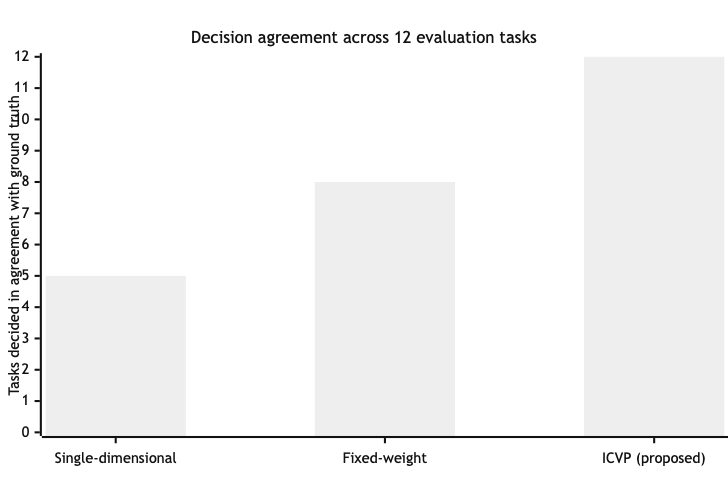
\includegraphics[width=0.75\columnwidth,height=0.72\textheight,keepaspectratio]{images/evaluation-headline.png}
    \caption{Decision agreement with the reference panel across the twelve evaluation tasks.}
    \label{fig:evaluation-headline}
\end{figure}

The fixed-weight baseline narrows the gap on tasks where the dominant intent is close to the implicit weights of the fixed profile, but it widens again on tasks where the intent reshapes which evidence matters and what the valuation dimensions mean. This pattern is consistent with the conceptual argument of Chapter \ref{sec:design}. Intent does not only change how much Availability, Durability, and Utility matter. It changes what counts as Availability, Durability, and Utility, and the fixed-weight baseline does not represent that change. If the final rerun preserves this paired pattern across decision quality, false-proceed rate, evidence relevance, mapping quality, trace completeness, and robustness conditions, then the evaluation supports the claim that ICVP is the better approach among the tested alternatives for this benchmark. The evaluation is not a proof that ICVP is the only adequate model, and we do not claim that the agentic implementation is correct in any stronger sense than the trace-gated authorisation property of Section \ref{sec:proof-targets} guarantees. The results indicate, however, that intent-conditioned projection and dimension instantiation, made auditable through valuation traces and validated by a deterministic check, may improve decision quality, evidence relevance, and auditability relative to the two reduced baselines on this benchmark.

The same body of results speaks to the operational claim made under RQ2. The full ICVP configuration produces traces that pass deterministic validation, record provenance, distinguish confident and deferred decisions, and link to prepared transactions inside the policy boundary of Section \ref{sec:onchain-layer}. The single-dimensional baseline does not pass validation because its trace omits intent-required evidence categories. The fixed-weight baseline passes validation but on a noisier evidence set. Validator rejection of the single-dimensional baseline is, in this context, a desirable property, because incomplete evidence is then prevented from flowing silently to authorisation.

The formal claim made under RQ1 is treated separately. The model of Section \ref{sec:icvp} and the proof targets of Section \ref{sec:proof-targets} are stated and argued by construction over an abstract state machine. The empirical evaluation in this chapter does not stand in for that argument. It does, however, exercise the model on tasks where the projection $P_i$ and the instantiation $\Phi_i$ are the load-bearing parts of the decision, and where the deterministic validator and human approval, rather than agentic confidence, are the binding constraints on authorisation.
